\chapter{Specyfikacja gramatyki}

% TODO 
% specyfikację gramatyki języka w notacji wybranego przez siebie narzędzia 
% wzorowane na Rozdziale 1 oraz Dodatku „Przewodnik języka C” (Sekcja „Gramatyka”) 
% książki „Język C”, B. Kernighan, D. Ritchie.

\section{Lexer}
Na listingu \ref{analiza-leksykalna-tokeny} zostały przedstawione tokeny obsługiwane przez nasz translator.

\begin{lstlisting}[language={Python}, caption={Analiza leksykalna - podział na tokeny}, label={analiza-leksykalna-tokeny}]
    tokens = (
        'AUTHOR',
        'BEGIN_DOCUMENT',
        'BEGIN_OLIST',
        'BEGIN_ULIST',
        'BEGIN_TABULAR',
        'BOLD',
        'CENTERLINE',
        'CHAPTER',
        'COLUMN_DIVIDER',
        'COLUMN_PATTERN_BORDERLESS',
        'COLUMN_PATTERN_BORDERED',
        'DOCUMENTCLASS',
        'END_DOCUMENT',
        'END_OLIST',
        'END_ULIST',
        'END_TABULAR',
        'GRAPHICS_PATH',
        'HLINE',
        'INCLUDE_GRAPHICS',
        'ITALIC',
        'ITEM',
        'LBRACE',
        'NEW_LINE',
        'NULL',
        'PARAGRAPH',
        'RBRACE',
        'ROW_END',
        'SECTION',
        'SUBSECTION',
        'SUBSUBSECTION',
        'TEXT',
        'TITLE',
        'UNDERLINE',
        'URL',
        'USE_PACKAGE',
    )
\end{lstlisting}

Tokeny na listingu \ref{analiza-leksykalna-tokeny} odpowiadają następującym wyrażeniom regularnym 
przedstawionym na listingu \ref{analiza-leksykalna-wyrazenia}:

\begin{lstlisting}[language={Python}, caption={Analiza leksykalna - wyrażenia regularne}, label={analiza-leksykalna-wyrazenia}]
    t_AUTHOR = r'\\author'
    t_BEGIN_DOCUMENT = r'\\begin\{document\}'
    t_BEGIN_OLIST = r'\\begin\{enumerate\}'
    t_BEGIN_ULIST = r'\\begin\{itemize\}'
    t_BEGIN_TABULAR = r'\\begin\{tabular\}'
    t_BOLD = r'\\textbf'
    t_CENTERLINE = r'\\centerline'
    t_CHAPTER = r'\\chapter'
    t_COLUMN_DIVIDER = r'&'
    t_COLUMN_PATTERN_BORDERLESS = r'\{[lcr](\s[lcr])*\}'
    t_COLUMN_PATTERN_BORDERED = r'\{(\|\s[lcr]\s)+\|\}'
    t_DOCUMENTCLASS = r'\\documentclass.*'
    t_END_DOCUMENT = r'\\end\{document\}'
    t_END_OLIST = r'\\end\{enumerate\}'
    t_END_ULIST = r'\\end\{itemize\}'
    t_END_TABULAR = r'\\end\{tabular\}'
    t_GRAPHICS_PATH = r'\\graphicspath'
    t_INCLUDE_GRAPHICS = r'\\includegraphics'
    t_ITALIC = r'\\textit'
    t_ITEM = r'\\item'
    t_LBRACE = r'\{'
    t_NEW_LINE = r'\\newline'
    t_NULL = r'\0'
    t_PARAGRAPH = r'\\paragraph'
    t_RBRACE = r'\}'
    t_ROW_END = r'\\\\'
    t_SECTION = r'\\section'
    t_SUBSECTION = r'\\subsection'
    t_SUBSUBSECTION = r'\\subsubsection'
    t_TEXT = r'[\w\d\.,!?@#/\'\"<>\(\)\-+=\/^\*:;|\[\]]+'
    t_TITLE = r'\\title'
    t_UNDERLINE = r'\\underline'
    t_URL = r'\\url'
    t_USE_PACKAGE = r'\\usepackage.*'
\end{lstlisting}

Definicje tokenów nowej linii, komentarza, błędów oraz tokenów ignorowanych zostały przedstawione na listingu \ref{analiza-leksykalna-pozostale}.

\begin{lstlisting}[language={Python}, caption={Analiza leksykalna - pozostałe tokeny}, label={analiza-leksykalna-pozostale}]
    def t_newline(self, t):
        r'\n+'
        t.lexer.lineno += t.value.count("\n")

    def t_comment(self, t):
        r'%.*\n'
        pass

    def t_hline(self, t):
        r'\\hline'
        pass

    t_ignore = ' '

    def t_error(self, t):
        print("Illegal character '%s'" % t.value[0])
        t.lexer.skip(1)
\end{lstlisting}

% 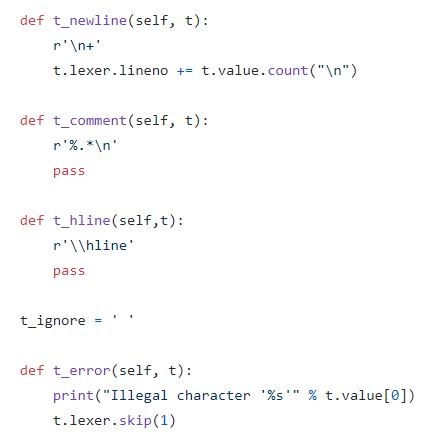
\includegraphics{tokens_def.JPG}

Należy zauważyć, że cała zawartość między znacznikiem "\textbf{\%}" w formacie \LaTeX, odpowiadającemu początkowi komentarza, do nowej linii, 
zostaje pominięta.

\section{Parser}

Każdy z dokumentów HTMLa musi zawierać znaczniki typowe dla tego formatu, których nie znajdziemy w dokumentach LaTeX. Są to: html,
head, body. Jako odpowienik sekcji head przyjęliśmy usepackage, a body odpowiada begin i end document.

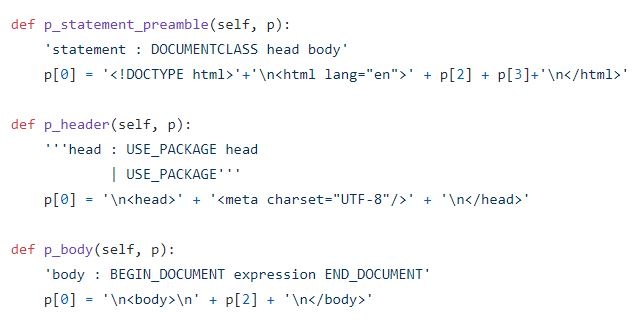
\includegraphics{preamble.JPG}

\subsection{Obsługa tekstu}

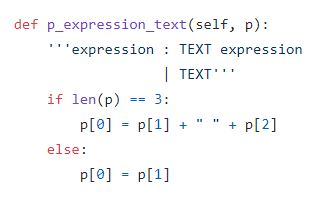
\includegraphics{expression_text.JPG}

\subsection{Formatowanie tekstu}

Nasz translator umożliwia pogrubienie, kursywa, podkreślenie, wyśrodkowanie tekstu oraz utworzenie paragrafu. Możliwe jest mieszanie
stylów formatowania, np. pogrubienie z podkreśleniem. Według nowych zaleceń, do pogrubienia tekstu w HTMLu powinno się stosować znacznik
"strong", a do kursywy "em".

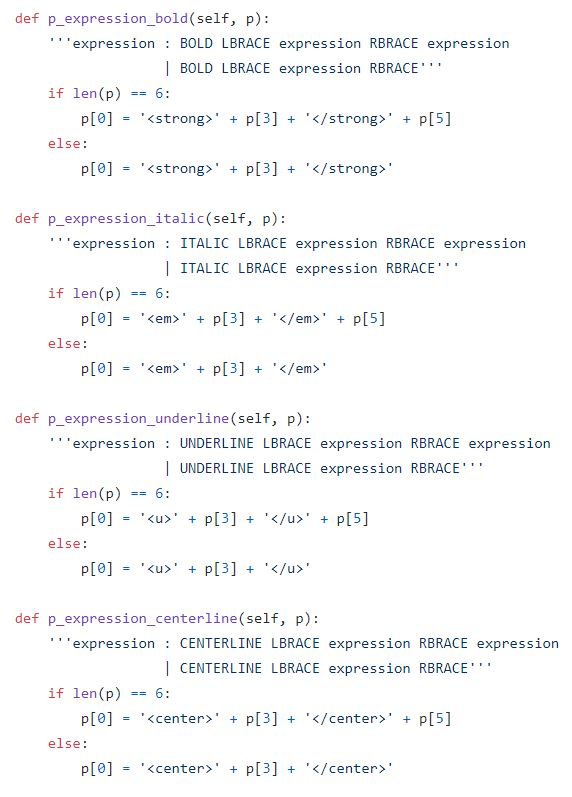
\includegraphics{bold_italic_underline_centerline.JPG}

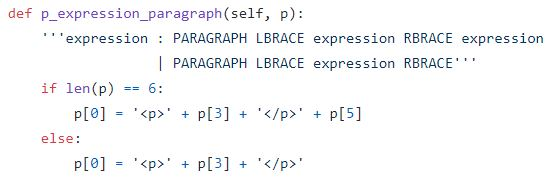
\includegraphics{paragraph.JPG}


Kolejną funkcjonalnością jest możliwość obsługi rozdziałów, sekcji i podsekcji parsując znaczniki chapter, section, subsection, 
subsubsection.


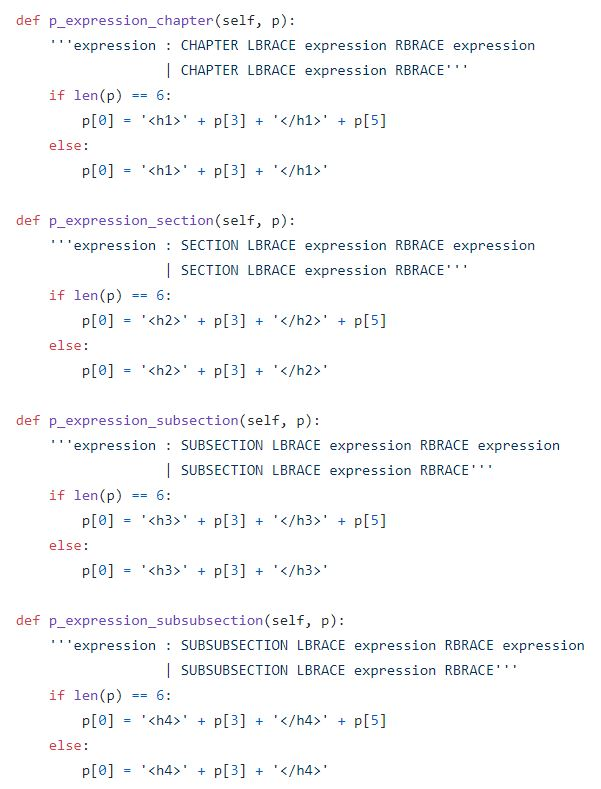
\includegraphics{chapter_section.JPG}


Przejście do nowej linii (hard break) jest obsłużony poleceniem newline.

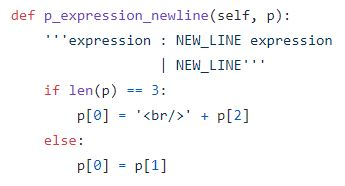
\includegraphics{newline.JPG}


Translator parsuje również znacznik title odpowiadjący z utworzenie tytułu.

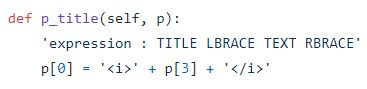
\includegraphics{title.JPG}

\subsection{Tabela}

\subsubsection{Z obramowaniem}

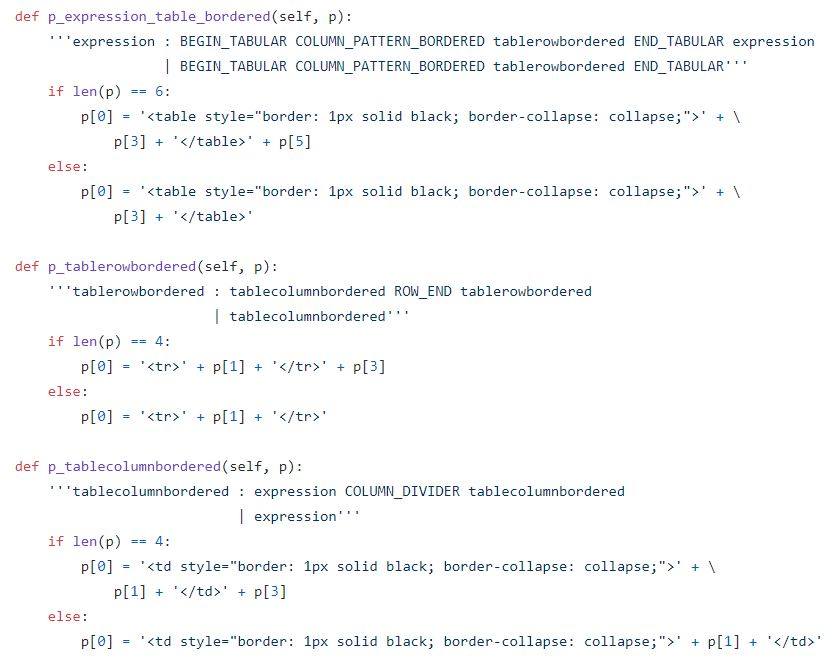
\includegraphics{table_bordered.JPG}

\subsubsection{Bez obramowania}

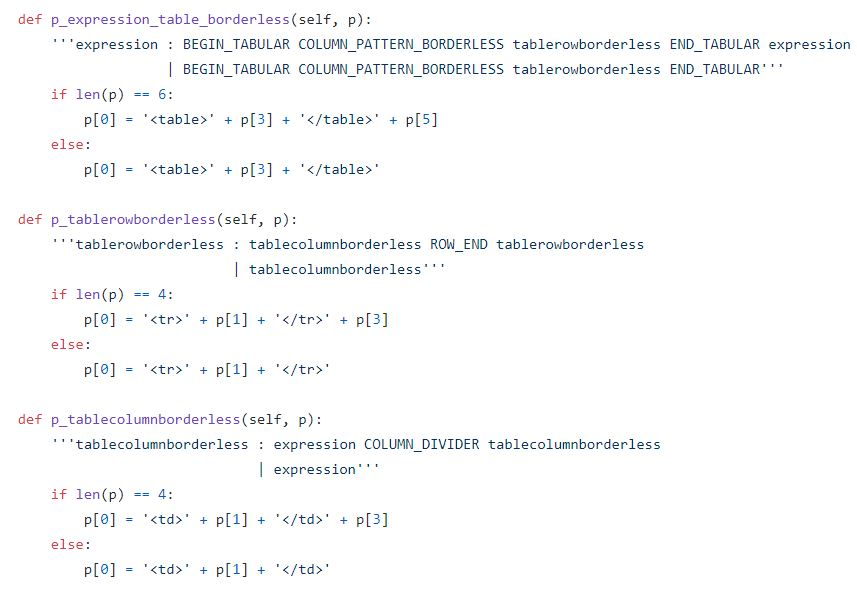
\includegraphics{table_borderless.JPG}


\subsection{Wyliczenie}

Konstrukcja parsera wyliczeń umożliwia wykonywanie zagnieżdżeń.

\subsubsection{Uporządkowane}

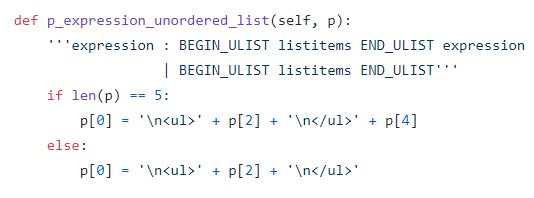
\includegraphics{unordered_list.JPG}

\subsubsection{Nieuporządkowane}

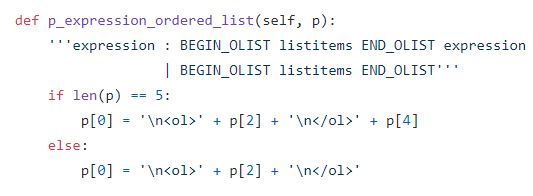
\includegraphics{ordered_list.JPG}

\subsection{Grafika}

Umieszcznie grafiki jest możliwe dzięki znacznikowi "includegraphics" w LaTeX, który jest parsowany na znacznik "img" w HTML, gdzie 
atrybut :src" stanowi ścieżka do pliku umieszczona w nawiasach wąsatych w dokumencie LaTeX.

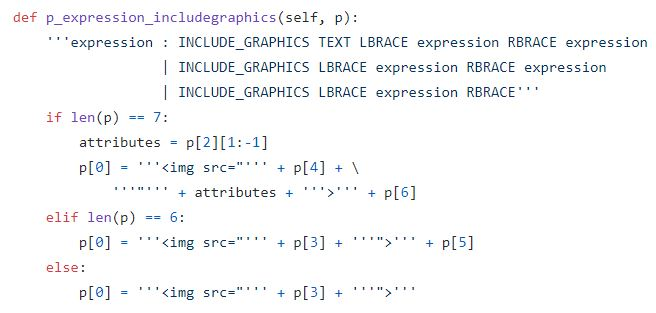
\includegraphics{includegraphics.JPG}

\subsection{Hiperłącze}

Zamieszczenie hiperłącza w formacie LaTeX jest możliwe dzięki znacznikowi "url", zawierającego w nawiasach wąsatych adres do strony.
Parsowanny jest on na HTMLowy znacznik "a" z atrybutem "href" zawierającego adres.

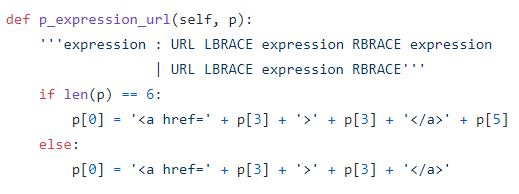
\includegraphics{url.JPG}